\documentclass{standalone}

\usepackage{tikz}
\usepackage{amsmath}
\usetikzlibrary{matrix}
\usetikzlibrary {shapes.geometric}
\usetikzlibrary {positioning}
\usetikzlibrary {decorations.pathmorphing}
\usetikzlibrary {arrows.meta}

\begin{document}
    
        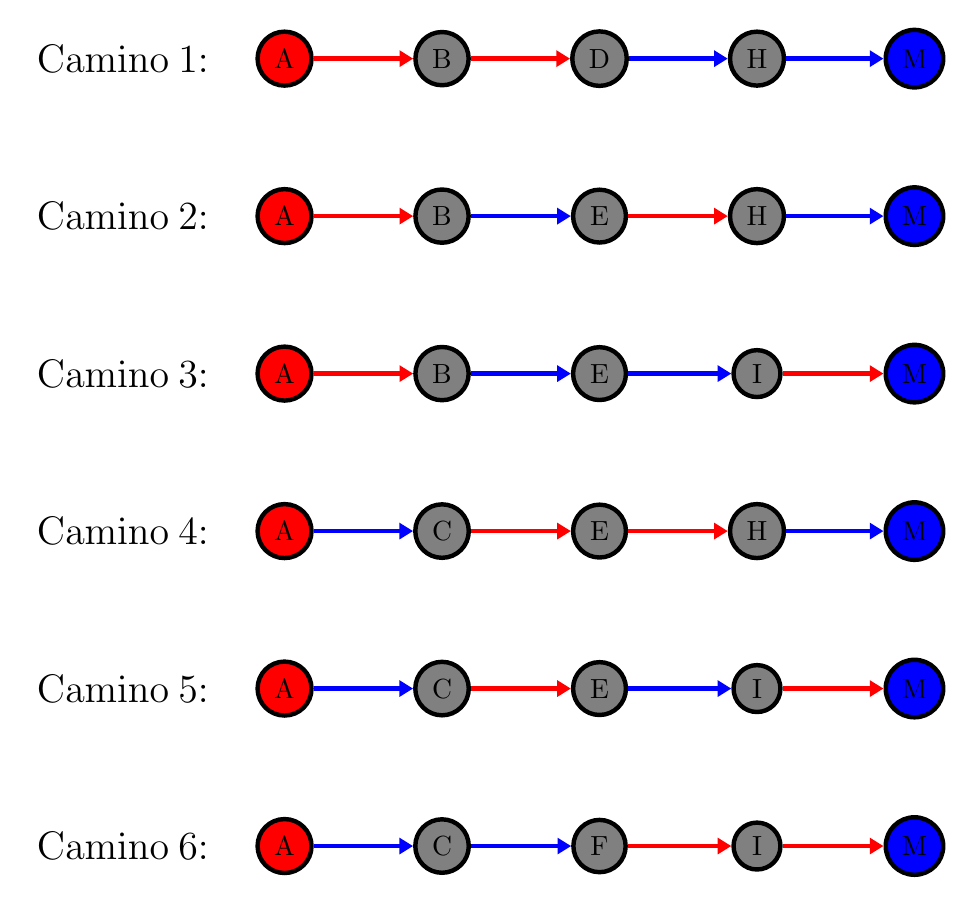
\begin{tikzpicture}[ultra thick]

            % \draw [help lines] (0,0) grid (8,12); 

            \path   (0,10) node (a) [circle,draw,fill=red] {A}
                    (2,10) node (b) [circle,draw,fill=gray] {B}
                    (4,10) node (c) [circle,draw,fill=gray] {D}
                    (6,10) node (d) [circle,draw,fill=gray] {H}
                    (8,10) node (e) [circle,draw,fill=blue] {M}
                    
                    (0,8) node (f) [circle,draw,fill=red] {A}
                    (2,8) node (g) [circle,draw,fill=gray] {B}
                    (4,8) node (h) [circle,draw,fill=gray] {E}
                    (6,8) node (i) [circle,draw,fill=gray] {H}
                    (8,8) node (j) [circle,draw,fill=blue] {M}

                    (0,6) node (k) [circle,draw,fill=red] {A}
                    (2,6) node (l) [circle,draw,fill=gray] {B}
                    (4,6) node (m) [circle,draw,fill=gray] {E}
                    (6,6) node (n) [circle,draw,fill=gray] {I}
                    (8,6) node (o) [circle,draw,fill=blue] {M}

                    (0,4) node (p) [circle,draw,fill=red] {A}
                    (2,4) node (q) [circle,draw,fill=gray] {C}
                    (4,4) node (r) [circle,draw,fill=gray] {E}
                    (6,4) node (s) [circle,draw,fill=gray] {H}
                    (8,4) node (t) [circle,draw,fill=blue] {M}

                    (0,2) node (u) [circle,draw,fill=red] {A}
                    (2,2) node (v) [circle,draw,fill=gray] {C}
                    (4,2) node (w) [circle,draw,fill=gray] {E}
                    (6,2) node (x) [circle,draw,fill=gray] {I}
                    (8,2) node (y) [circle,draw,fill=blue] {M}

                    (0,0) node (uz) [circle,draw,fill=red] {A}
                    (2,0) node (vz) [circle,draw,fill=gray] {C}
                    (4,0) node (wz) [circle,draw,fill=gray] {F}
                    (6,0) node (xz) [circle,draw,fill=gray] {I}
                    (8,0) node (yz) [circle,draw,fill=blue] {M};
                    




                    
                
            \draw[arrows = -{Triangle[open, angle=60:2mm,fill=red]},red] (node cs: name =a ) -- (node cs:name =b);
            \draw[arrows = -{Triangle[open, angle=60:2mm,fill=red]},red] (node cs: name =b ) -- (node cs:name =c);
            \draw[arrows = -{Triangle[open, angle=60:2mm,fill=blue]},blue] (node cs: name =c ) -- (node cs:name =d);
            \draw[arrows = -{Triangle[open, angle=60:2mm,fill=blue]},blue] (node cs: name =d) -- (node cs:name =e);
            
            \draw[arrows = -{Triangle[open, angle=60:2mm,fill=red]},red] (node cs: name =f ) -- (node cs:name =g);
            \draw[arrows = -{Triangle[open, angle=60:2mm,fill=blue]},blue] (node cs: name =g ) -- (node cs:name =h);
            \draw[arrows = -{Triangle[open, angle=60:2mm,fill=red]},red] (node cs: name =h ) -- (node cs:name =i);
            \draw[arrows = -{Triangle[open, angle=60:2mm,fill=blue]},blue] (node cs: name =i ) -- (node cs:name =j);
            
            \draw[arrows = -{Triangle[open, angle=60:2mm,fill=red]},red] (node cs: name =k ) -- (node cs:name =l);
            \draw[arrows = -{Triangle[open, angle=60:2mm,fill=blue]},blue] (node cs: name =l ) -- (node cs:name =m);
            \draw[arrows = -{Triangle[open, angle=60:2mm,fill=blue]},blue] (node cs: name =m) -- (node cs:name =n);
            \draw[arrows = -{Triangle[open, angle=60:2mm,fill=red]},red] (node cs: name =n ) -- (node cs:name =o);

            \draw[arrows = -{Triangle[open, angle=60:2mm,fill=blue]},blue] (node cs: name =p ) -- (node cs:name =q);
            \draw[arrows = -{Triangle[open, angle=60:2mm,fill=red]},red] (node cs: name =q ) -- (node cs:name =r);
            \draw[arrows = -{Triangle[open, angle=60:2mm,fill=red]},red] (node cs: name =r) -- (node cs:name =s);
            \draw[arrows = -{Triangle[open, angle=60:2mm,fill=blue]},blue] (node cs: name =s ) -- (node cs:name =t);

            \draw[arrows = -{Triangle[open, angle=60:2mm,fill=blue]},blue] (node cs: name =u ) -- (node cs:name =v);
            \draw[arrows = -{Triangle[open, angle=60:2mm,fill=red]},red] (node cs: name =v ) -- (node cs:name =w);
            \draw[arrows = -{Triangle[open, angle=60:2mm,fill=blue]},blue] (node cs: name =w) -- (node cs:name =x);
            \draw[arrows = -{Triangle[open, angle=60:2mm,fill=red]},red] (node cs: name =x ) -- (node cs:name =y);

            \draw[arrows = -{Triangle[open, angle=60:2mm,fill=blue]},blue] (node cs: name =uz ) -- (node cs:name =vz);
            \draw[arrows = -{Triangle[open, angle=60:2mm,fill=blue]},blue] (node cs: name =vz ) -- (node cs:name =wz);
            \draw[arrows = -{Triangle[open, angle=60:2mm,fill=red]},red] (node cs: name =wz) -- (node cs:name =xz);
            \draw[arrows = -{Triangle[open, angle=60:2mm,fill=red]},red] (node cs: name =xz ) -- (node cs:name =yz);
            
            \node [left=1cm,text width=2cm] at (a)
            {
            \mbox{\Large Camino 1:}
            };

            \node [left=1cm,text width=2cm] at (f)
            {
            \mbox{\Large Camino 2:}
            };

            \node [left=1cm,text width=2cm] at (k)
            {
            \mbox{\Large Camino 3:}
            };

            \node [left=1cm,text width=2cm] at (p)
            {
            \mbox{\Large Camino 4:}
            };

            \node [left=1cm,text width=2cm] at (u)
            {
            \mbox{\Large Camino 5:}
            };

            \node [left=1cm,text width=2cm] at (uz)
            {
            \mbox{\Large Camino 6:}
            };
        \end{tikzpicture}
\end{document}